%! TEX root = ../supernova_2023.tex
\documentclass[supernova_2023]{subfiles}
\begin{document}
\chapter{星空写真の始め方}
\rightline{3年 森山陽介}
私が星空写真を始めたときに躓いたところを細かく説明しながら簡単に星が撮れることを説明しようと記事を書いていたらとても長く,まとまりがつかなくなったので,いくつか割愛・抜粋して付録としてお届けします。別の機会にすべてお伝えできたらいいなと考えています。
\section{星空写真の種類}
星空をメインにした写真には大きく分けて次の3種類が挙げられます。
\subsection{星景写真}
\begin{itemize}
  \item 広角で星空と風景の両方の写真が写っている写真のこと
  \item 比較的撮影の難易度が低い
  \item カメラと三脚があれば今すぐにでも試せる
\end{itemize}
\subsection{星野写真}
\begin{itemize}
  \item 標準~中望遠程度の画角で星空のみ,星座などが中心の写真
  \item ISO感度を上げればカメラと三脚だけでも撮れないことはない。
  \item 本格的に撮るとなると,ポータブル赤道儀など専門的な機材が必要
\end{itemize}
\subsection{天体写真}
\begin{itemize}
  \item 望遠~超望遠で惑星や星雲・銀河などが主役になる写真
  \item 赤道儀と天体望遠鏡が必須
  \item 撮影方法やその後の処理含めて必要な機材が多くて複雑
\end{itemize}
\section{初心者はまず星景写真から}
星空観測を楽しむためには、天体望遠鏡が必要だと考える人も多いでしょう。天体望遠鏡を使えば月や惑星、星雲や銀河などを観察したり撮影することができます。しかし、そういった天体望遠鏡は非常に高価だったり、よく選ばずに安価なものを買うと何も見えず満足に楽しめないこともあり初心者には特にハードルが高く感じるでしょう。そのため、まずは手軽に星空観測を楽しむ方法として、カメラと三脚さえあれば始められる星景写真を紹介します。

星景写真は、広角レンズを使用して、星空と風景を一緒に写した写真です。星空観測と同様に、撮影する場所や時間帯が重要です。また、カメラの設定が重要で、マニュアルモードでの撮影がおすすめです。露出時間やISO感度、絞りなどを調整することで、美しい星空写真を撮影することができます。

\begin{tcolorbox}[title=星景写真に必要な物, breakable]
  \begin{description}
    \item[カメラ:]この後にも詳しく説明しますが、マニュアル設定ができるカメラが必要です。
    \item[三脚:]長時間露光をするために、カメラを固定する三脚が必要です。なるべく脚が太くて耐荷重の大きい物が良いです。特にカーボン製でセンターポールのないものがおすすめ。
    \item[リモートシャッター:]リモートシャッターを使用することで、カメラを手で触ることなくシャッターを切ることができます。三脚を使っていても、長時間露光をする星景写真では、シャッターボタンを直接押して撮影するのは被写体ブレにつながってしまいます。リモコンやスマホなどでシャッターを切るか、タイマー機能を利用しましょう。
    \item[星空観望の必需品] \mbox{}\\
    \begin{description}
      \item[防寒具:] 外で長時間過ごすため、防寒具が必要です。星景写真を撮影する場合、晴れた夜空の下では放射冷却によって地面から冷気が上がってくるように寒くなります。家を出るときは着すぎず、汗ばむ程度がちょうどいいです。ただし、汗ばんだままだと体温を下げてしまうので、服選びでは保温性に加えて透湿性にも注意しましょう。足元が冷たくなるため、スノーブーツと雪用靴下を履くことをおすすめします。\mbox{}\par
      例えば、肌着にエアリズムを着用し、厚手のヒートテック、フリース、そしてダウンを重ね着することで、防寒性を高めながら透湿性も確保することができます。ただし、着込みすぎても熱が奪われてしまうため、適度な空気の層を取り込んでおくことが大切です。着込みすぎると動きにくく、むしろ熱が奪われやすくなります。
      \item[ヘッドランプ:] 夜間に撮影する場合、手元が暗くなるため、ヘッドランプが必要です。ヘッドランプを使用することで、手元を照らし、操作をスムーズに行うことができます。(赤色か電球色の弱めのライトがおすすめ:暗順応)
      \item[行動食:] 星空観望の一番の敵は真夜中の寒さです。防寒着ももちろん大切ですが、体の内側から熱を生み出すために軽食や水分の補給も必要です。チョコを含んだお菓子や温かい紅茶などを準備していくといいでしょう。
      \item[スマートフォン:] 星座表や懐中電灯代わりにもなりますし、非常時の連絡や地図の確認などで必要不可欠です。また、星空撮影では撮影の間かなり暇を持て余すので暇つぶしにも必要です。
    \end{description}
      \centering
      \includegraphics[width=8cm]{figures/Yosuke/iMG_.png}
  \end{description}
\end{tcolorbox}

\section{星空を撮るためのカメラ 必要なスペックは?}
星空を撮るために必要最小限のスペックは
\begin{description}
  \item[マニュアル露出:] シャッター速度、F値、ISO感度のそれぞれが独立して設定できること
  \item[マニュアルフォーカス:]レンズのピントを手動で合わせることができること
\end{description}
です。一般的にこれができる一眼レフやミラーレス一眼(以下:一眼)であればどれを選んでも星を撮ることはできます。さらに以下の機能が備わっているとより快適に撮影に臨むことができます。
\begin{description}
  \item[ライブビュー機能:] カメラが撮る構図を背面ディスプレイでモニターできる機能
  \item[バリアングル液晶:] カメラの設置位置や構図によっては背面液晶を見るのが苦しい場面もあるので、この機能があるととても楽です。
  \item[USB給電:] 星空の撮影は長時間に及ぶことが多いので、予備の電池やDCカプラーなどが必要なことがありますが、USB給電ができるカメラなら、手持ちのモバイルバッテリーとケーブルでカメラを給電しながら撮影できます。(USB充電ではないことに注意!)
  \item[リモコン端子:] 有線のリモコン(タイマーレリーズ)を取り付けることができること。無線のリモコンやインターバル撮影機能があればそれでもよいが、後の拡張性を考えると有線が取り付けられる方がいい。シャッターのタイマー機能でも代用はできる。有線のタイマーレリーズとしては「ROWA JAPAN」のものが有名でよく使われています。
  \item[防塵防滴構造:] 星空撮影は完全アウトドアな撮影です。ロケ地によっては砂埃が舞うこともあれば、夜露で明け方にはびしょびしょになることもあります。あってもダメになるときはありますが、ないよりは安心です。
  \item[センサーゴミ取り機能:] 屋外でレンズ交換や、望遠鏡に取り付けるときはセンサーが外気と直接触れる場面もあります。自分で清掃する必要がある時もありますが、この機構があればその機会も減らせると思います。      
\end{description}
\begin{tcolorbox}[title=一眼じゃなきゃダメ?, breakable]
  最近のスマートフォンなどでも綺麗な星景写真を撮ることは十分可能で,意外と手軽に星空を写せる時代にもなりました。Xperia 5やXperia 1では標準でマニュアル露出やマニュアルフォーカスの機能が備わっているので、タイマー撮影で星景写真を取ることも可能です。\footnote{だから私はXperia。}また、PixelやiPhoneなどはマニュアル撮影ができなくても自動で星空を認識して最適な設定で撮影できたりします。しかし、そういったスマートフォンやコンパクトデジタルカメラは上位機種に限られ、同じ価格で一眼を一台かそれ以上買えたりすることもあります。星空が撮れるといっても、一眼とスマホとでは画質やその後の拡張性に大きな違いがあります。そういった点から星空の撮影を始めるなら一眼を手に入れることをおすすめします。
\end{tcolorbox}
\section{準備ができたら早速撮影しに行ってみよう!}
必要な物をそろえたら,荷物を持って空が開けた場所に行って撮影をしてみましょう。カメラの写真の保存設定をRAWに,シャッター速度を$200 / \text{(使っているレンズの焦点距離)}$で求めた値(200ルール)より大きくならないことに気をつければ,後はどうにかなります。最初はピントを合わせるのが大変だと思いますが,ライブビューで拡大してみたり,遠くの夜景にオートフォーカスで合わせてマニュアルにして固定しておくなどすればできると思います。とにかく実践あるのみです。
\begin{figure}
  \centering
  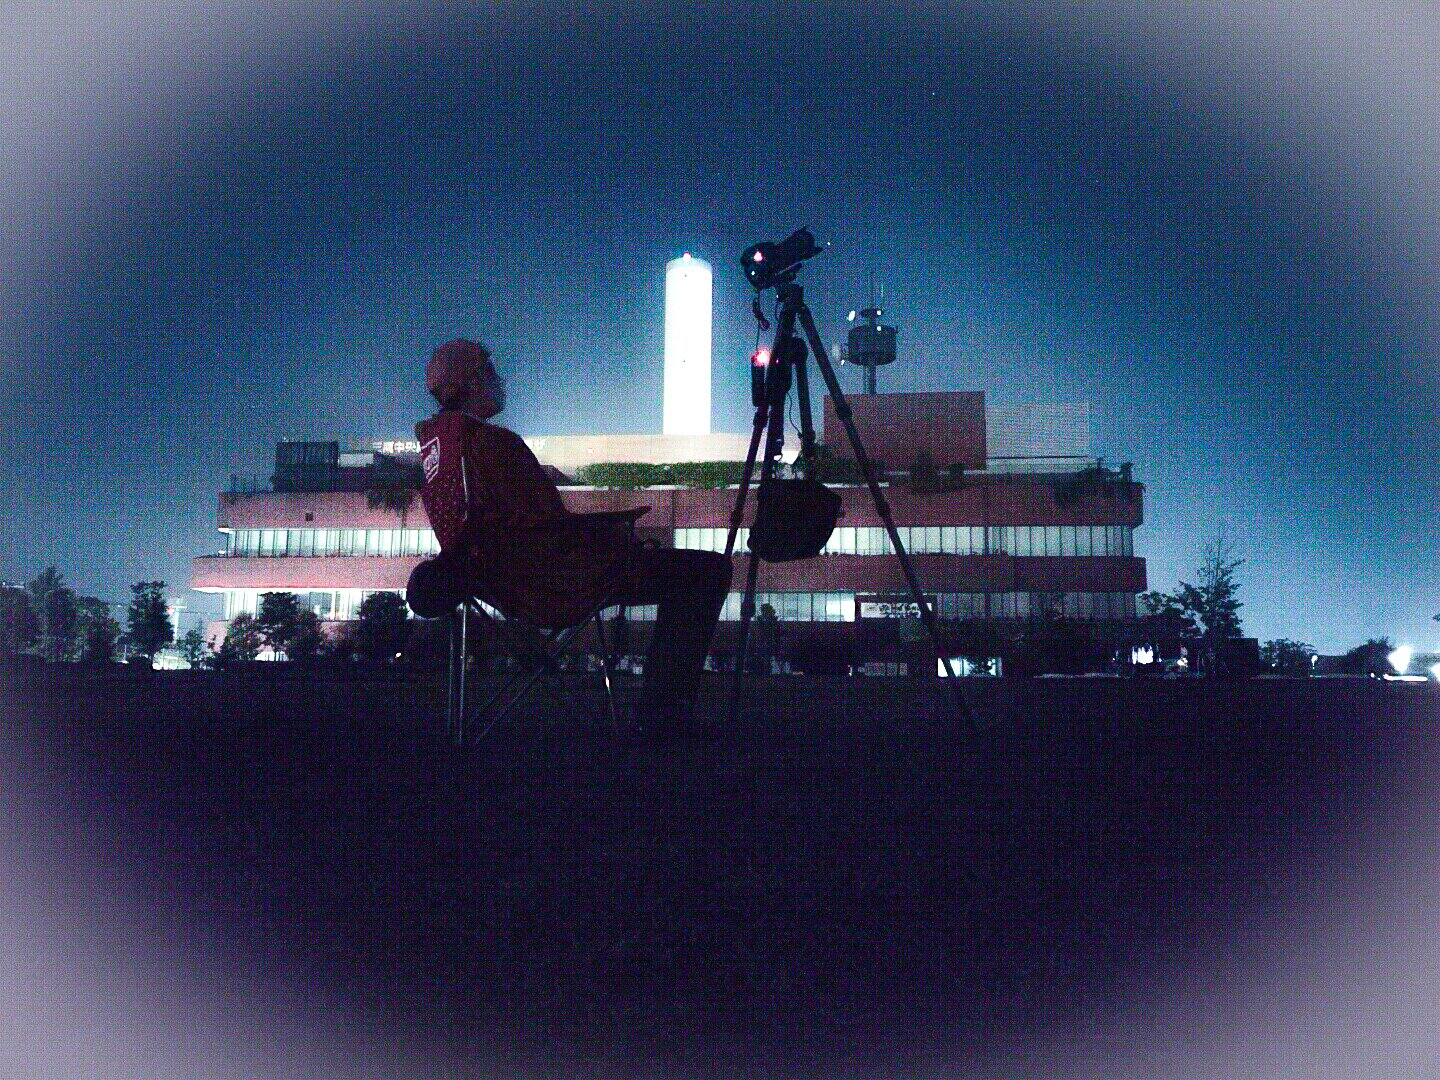
\includegraphics[width=8cm]{figures/Yosuke/Hitori.jpg}
  \caption{カメラを設置して星空撮影会}
  \label{fig:Hitori}
\end{figure}
\begin{tcolorbox}[title=星空観望・撮影をいつする?, breakable]
  星空観望・撮影をするにあたり、まずは天気の確認が必要です。天気が悪いと星空が見えにくく、撮影も難しくなってしまいます。月齢や天気などを気にする必要があります。月齢が満月の頃は、月の明かりで星空が見えにくくなってしまいます。逆に、新月の頃は月の明かりが少ないため、星空をより美しく見ることができます。また、天気に関しては雲量の確認が重要であるため、SCW天気予報やWindyなどのサイトを確認することがいいとされています。これらのサイトでは、天気予報だけでなく、雲量や風向き、湿度などの情報も確認することができます。
  
  \phantom{a}\par
  次に、観望や撮影のスポットに関してです。スポット選びには、見晴らしがいいこと、光害の影響が少ないこと、トイレなどが近くにあることが重要視されます。星空を見るためには、周りに明かりが少ない場所がいいでしょう。都市部では光害がひどく、星空を見ることができない場合があります。光害汚染マップや青宙スポットなどを確認することで、星空を楽しめるスポットを探すことができます。また、キャンプ場や自然公園なども星空を楽しむには適したスポットです。トイレや駐車場が近くにあるかどうかも確認することが大切です。
  
  \phantom{a}\par 
  最後に、星空観望・撮影をする場合は、自然を守ることが大切です。星空観測をする場合は、ゴミの持ち帰りや、周囲の環境への配慮を心がけましょう。星空観測を楽しみながら、自然を守ることができるように、心がけていきましょう。
\end{tcolorbox}
\section{さいごに}
カメラの露出設定は日によって様々なので,この場で伝えるのが難しいですが,もっと初心者向きな方法として,星が動く軌跡の写真を作ったり,タイムラプス動画を作ってみるなどがあります。

カメラを設置したら最低2~3時間程度動かさずに連続でシャッターを切り続けて行くことで素材を集めていきましょう。このとき,シャッター速度は20秒~30秒,F値は一番小さい値,ISOは100あたりで撮っておいても問題ありません。こうしてたくさんの同じ構図の連続写真が撮れたら,Windowsの人は「SiriusComp」というフリーソフト,Macの人は「StarStaX」というフリーソフトを使って星の軌跡写真を作ってみましょう。特に「SiriusComp」は軌跡写真と同時にタイムラプス動画も作ってくれるのでとてもおすすめです。星の軌跡写真は「比較明合成」という手法を用いているので,できる人はPythonなどで自分で処理してみるのもいいと思います。

ちなみに,私が撮りためたタイムラプスをまとめた動画をYouTubeで公開しています。左下に撮影情報も載せているので,よかったら参考にしてみてください。(ピンぼけのもいくつかありますが\^\^;)
\begin{figure}[H]
  \centering
  \begin{minipage}{0.4\columnwidth}
    \centering
    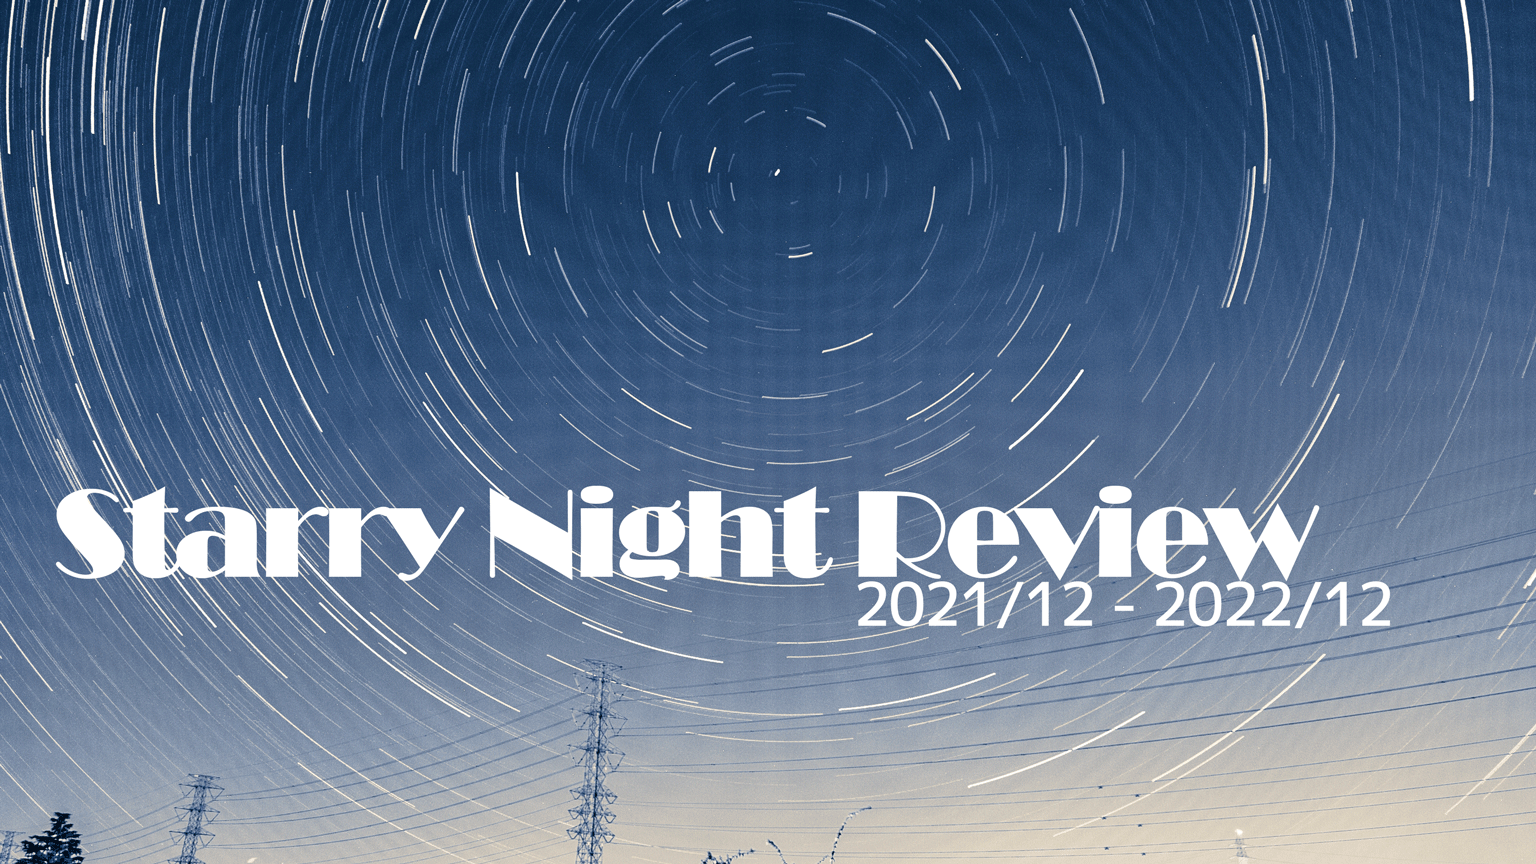
\includegraphics[width=.8\columnwidth]{figures/Yosuke/Starry_Night_Review_thumbnail.png}
    \caption{2022年をまとめたタイムラプス動画}
    \label{fig:starry}
  \end{minipage}
  \begin{minipage}{0.4\columnwidth}
    \centering
    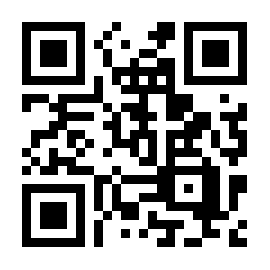
\includegraphics[width=.5\columnwidth]{figures/Yosuke/QR_031871.png}
    \caption{YouTube動画はこちらから}
    \label{fig:QR}
  \end{minipage}
\end{figure}

\begin{thebibliography}{1}
  \bibitem{nari} 成澤広幸,成澤広幸の星空撮影塾 決定版,双葉社,2021年
  \bibitem{digi} デジタルカメラマガジン,2022年9月号,インプレス,2021年
\end{thebibliography}
\end{document}